\documentclass[]{article}

\input{MyTools}
\usepackage{physics}
\usepackage{changepage}
\usetikzlibrary{patterns}

\tikzset{
  oblique lines/.style={
    pattern = north east lines,
    pattern color = red,
  }
}
\begin{document}
\thispagestyle{empty}
\begin{figure}
    \begin{minipage}{0.7\textwidth}
        \begin{tabular}{l l}
            Department   & : Mathematics and Computer Science \\
            Level        & : Third Level                      \\
            Course Code  & : 040101309                        \\
            Course Title & :  Integral Equations              \\
            Semester     & : Fall 2023                        \\
            Time Allowed & : 30 minutes                       \\
            Lecturer     & : Dr.Hanna R. Ebead                \\
            Total Marks  & : 30 Points                        \\
        \end{tabular}
    \end{minipage}%
    \begin{minipage}{0.3\textwidth}
        \includegraphics[width=4.5cm]{collagelogo.png}
    \end{minipage}
\end{figure}
\vspace*{-1cm}
\begin{center}
    \textbf{\underline{\LARGE Mid-Term Examination-Model Answer}}
\end{center}
\vspace*{.2cm}

\hrule
\textbf{[10 marks]}\\
\textbf{\underline{Question 1: (a)}}
\begin{adjustwidth}{1cm}{2cm}
    Using \textit{Successive Approximation Method}\\
    Let initial guess $\displaystyle y_{o}(t) =x$ Then
    \begin{align*}
        y_1(t) & = x -\int_0^x (x-t)t \, dt = x-\frac{x^3}{3!}                                                                                                \\
        y_2(t) & = x -\int_0^x (x-t)(t-\frac{t^3}{3!})\, dt = x-\frac{x^3}{3!}+\frac{x^5}{5!}                                                                 \\
        y_3(t) & = x-\frac{x^3}{3!}+\frac{x^5}{5!}-\frac{x^7}{7!}                                                                                             \\
        \vdots &                                                                                                                                              \\
        y_n(t) & =x-\frac{x^3}{3!}+\frac{x^5}{5!}-\frac{x^7}{7!}+\dots+ \frac{(-1)^{n-1}x^{2n+1}}{(2n+1)!} = \sum_{k=1}^{n}\frac{(-1)^{k-1}x^{2k+1}}{(2k+1)!} \\
    \end{align*}
    Since $\displaystyle y(x) = \lim_{n \to \infty} y_n(t)$ we deduce that
    \begin{align*}
        y(t) & =\lim_{n \to \infty}\sum_{k=1}^{n} \frac{(-1)^{n-1}x^{2n+1}}{(2n+1)!} \\
             & =\sum_{k=1}^{\infty} \frac{(-1)^{n-1}x^{2n+1}}{(2n+1)!} = \sin(x)
    \end{align*}
\end{adjustwidth}
%==========================================================================

\textbf{\underline{Question 1: (b)}}
\begin{adjustwidth}{1cm}{2cm}
    Since $k(t,s)=ts  \,$ separable, we can use \textit{Direct Computational Medthod}\\
    \begin{equation*}
        y(t) = \frac{7}{8}t + \frac{1}{2}t \int_0^1 ts y^2(s) \, ds
    \end{equation*}
    Let $\displaystyle C :=\int_0^1 s y^2(s) \, ds$
    \begin{align*}
        y(t) & = \frac{7}{8}t + \frac{1}{2}tC                                                                                       \\
        C    & = \int_0^1 s \left[\frac{7}{8}s + \frac{1}{2}sC\right]^2 \,ds                                                        \\
        C    & = \int_0^1 s^3 \left[\frac{7}{8} + \frac{1}{2}C\right]^2 \,ds = \frac{1}{4}\left[\frac{7}{8} + \frac{1}{2}C\right]^2 \\
    \end{align*}
    \begin{equation*}
        16C^2 -200C+49=0
    \end{equation*}
    We get two solutions
    \[
        \begin{cases}
            \displaystyle y_1(t) = 7t \quad \text{At} \quad C_1 = \frac{49}{4} \\\\
            \displaystyle y_2(t) = t \quad \text{At}  \quad C_2 = \frac{1}{4}  \\
        \end{cases}
    \]
\end{adjustwidth}
%==========================================================================
\textbf{[10 marks]}\\
\textbf{\underline{Question 2: (a)}}
\begin{adjustwidth}{1cm}{2cm}
    Since $k$ is continuous on a closed domain $[a,b]\times[a,b]$. so it guarantees the existence of a finite  $L>0$\\
    From \textit{Existence and uniqueness theorem} we are able to prove that the integral equation has a unique continuous solution $y\in C[a,b]$\\
    Since
    $$f,k(t,.) \in C[a,b] \subset L_2[a,b] \quad,\quad t \in [a,b]$$\\
    Then
    $$M = \int_a^b \int_a^b |k(t,s)|^2 \, ds dt \leq \int_a^b \int_a^b L^2 \, ds dt = L^2 (b-a)^2 $$
    $$\sqrt{M} \leq L(b-a)$$
    Thus, we deduce that
    $$|\lambda|\,< \frac{1}{\sqrt{M}} \rightarrow |\lambda|\,< \frac{1}{L(b-a)}$$
\end{adjustwidth}
%==========================================================================
\textbf{\underline{Question 2: (b)}}
\begin{adjustwidth}{1cm}{2cm}
    Consider the Integral Equation
    \[
        y(t) = -4 + \int_{0}^{1}(2t+3s)y(s) \,ds \quad,\quad  t \in [0,1]
    \]
    We have $\lambda = 1$ , $L = \max\limits_{t,s\in [a,b]\times[a,b]} |2t+3s| = 5$ , $b-a = 1$
    which means that it doesn't satisfy the theorem because $\displaystyle |\lambda|< \frac{1}{L(b-a)}$ doesn't hold
    \\
    But  the equation has an exact solution given by $y(t) = 4t$
\end{adjustwidth}
%==========================================================================
\textbf{[10 marks]}\\
\textbf{\underline{Question 3:}}
\begin{adjustwidth}{1cm}{2cm}
    Let $y$ solves the IVP.\\
    Integerate the equation from $0 \to x$
    \begin{equation}
        \int_{0}^{x} y''(t) \, dt -2\underbrace{\int_{0}^{x} t y'(t) \,dt}_J -3\int_{0}^{x}y(t) \,dt=0
    \end{equation}
    Using integeration by parts on $J$ we get
    \begin{align*}
        J & := \int_{0}^{x} t y'(t) \,dt = \left[t y(t)\right]_{0}^{x} - \int_{0}^{x}y(t) \,dt= xy(x) - \int_{0}^{x}y(t) \,dt \\
    \end{align*}
    Subtitute in (1)
    \begin{align*}
        y'(x) - y'(0) -2xy(x) + 2\int_{0}^{x}y(t) \,dt -3\int_{0}^{x}y(t) \,dt & =0
        \\
        y'(x) -2xy(x) -\int_{0}^{x}y(t) \,dt                                   & =0 \tag{2}
    \end{align*}

    Integerate (2) from $0 \to x$
    \\
    %\begin{figure*}[h]
    \begin{minipage}{0.7\textwidth}
        \begin{align*}
            y(x) & -y(0) -2\int_{0}^{x}ty(t)\,dt -\int_{0}^{x}\int_{0}^{\xi}y(t) \, dtd\xi=0
            \\
            y(x) & = 1 +2\int_{0}^{x}ty(t)\,dt +\int_{0}^{x}\int_{t}^{x}y(t) \, d\xi dt
            \\
            y(x) & = 1 +2\int_{0}^{x}ty(t)\,dt +\int_{0}^{x}(x-t)y(t)dt
            \\
            y(x) & = 1 +\int_{0}^{x}(x+t)y(t)dt
        \end{align*}
    \end{minipage}%
    \begin{minipage}{0.3\textwidth}
        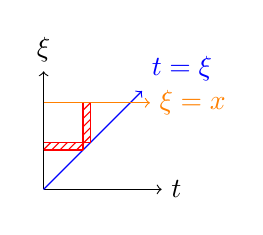
\begin{tikzpicture}[scale=0.5]
            \draw[->] (0,0,0) -- (3,0,0) node[right]{$t$};
            \draw[->] (0,0,0) -- (0,3,0) node[above]{$\xi$};
            \draw[->, blue] (0,0,0) -- (2.5,2.5,0) node[above right]{$t = \xi $};
            \draw[->, orange] (0,2.2,0) -- (2.7,2.2,0) node[right]{$\xi = x$};

            \draw[-,red] (0,1,0)--(1,1,0);
            \draw[-,red] (0,1.2,0)--(1.2,1.2,0);

            \fill [oblique lines] (0,1,0) -- (1,1,0) -- (1.2,1.2,0) -- (0,1.2,0);
            \fill [oblique lines] (1,1,0) -- (1,2.2,0) -- (1.2,2.2,0) -- (1.2,1.2,0);

            \draw[-,red] (1,1,0)--(1,2.2,0);
            \draw[-,red] (1.2,1.2,0)--(1.2,2.2,0);
        \end{tikzpicture}
    \end{minipage}
    %\end{figure*}
\end{adjustwidth}
%==========================================================================





\end{document}